% !TEX root = ../main.tex
% The god and the family trees: framing worlds (left) and growing worlds (right).
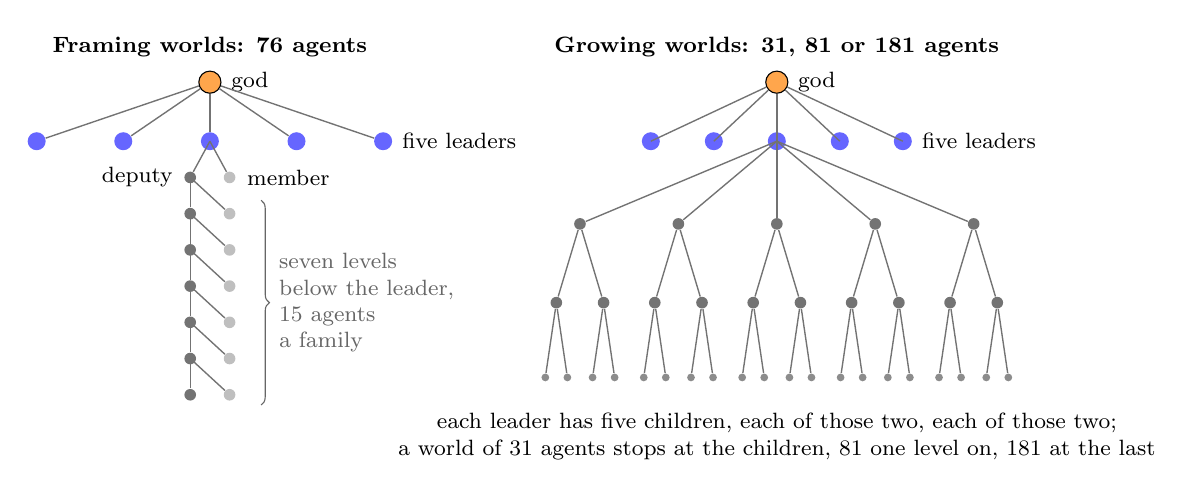
\begin{tikzpicture}[
  every node/.style={font=\footnotesize},
  agent/.style={circle, fill=black!55, inner sep=0, minimum size=4.2pt},
  member/.style={circle, fill=black!25, inner sep=0, minimum size=4.2pt},
  tiny/.style={circle, fill=black!45, inner sep=0, minimum size=2.8pt},
  top/.style={circle, draw=black, fill=orange!70, inner sep=0, minimum size=8pt},
  lead/.style={circle, fill=blue!60, inner sep=0, minimum size=6.5pt},
  edge/.style={black!55, line width=0.5pt},
]
% ---- framing worlds ----
\node[font=\footnotesize\bfseries] at (2.8,4.75) {Framing worlds: 76 agents};
\node[top, label={right:god}] (g) at (2.8,4.3) {};
\foreach \x/\n in {0.6/a,1.7/b,2.8/c,3.9/d,5.0/e} {
  \node[lead] (\n) at (\x,3.55) {};
  \draw[edge] (g) -- (\n);
}
\node[anchor=west] at (5.12,3.55) {five leaders};
\coordinate (prev) at (c);
\foreach \i in {1,...,7} {
  \pgfmathsetmacro{\y}{3.55-0.46*\i}
  \node[agent] (dep\i) at (2.55,\y) {};
  \node[member] (mem\i) at (3.05,\y) {};
  \draw[edge] (prev) -- (dep\i);
  \draw[edge] (prev) -- (mem\i);
  \coordinate (prev) at (dep\i);
}
\node[anchor=east] at (2.45,3.09) {deputy};
\node[anchor=west] at (3.15,3.09) {member};
\draw[decorate, decoration={brace, amplitude=3pt}, black!60] (3.45,2.8) -- (3.45,0.2) node[midway, right=3pt, align=left] {seven levels\\below the leader,\\15 agents\\a family};
% ---- growing worlds ----
\node[font=\footnotesize\bfseries] at (10.0,4.75) {Growing worlds: 31, 81 or 181 agents};
\node[top, label={right:god}] (G) at (10.0,4.3) {};
\foreach \x in {8.4,9.2,10.0,10.8,11.6} {
  \node[lead] at (\x,3.55) {};
  \draw[edge] (G) -- (\x,3.55);
}
\node[anchor=west] at (11.72,3.55) {five leaders};
\foreach \i in {0,...,4} {
  \pgfmathsetmacro{\cx}{10.0+(\i-2)*1.25}
  \node[agent] (c\i) at (\cx,2.5) {};
  \draw[edge] (10.0,3.55) -- (c\i);
  \foreach \j in {0,1} {
    \pgfmathsetmacro{\gx}{\cx+(\j-0.5)*0.6}
    \node[agent] (g\i\j) at (\gx,1.5) {};
    \draw[edge] (c\i) -- (g\i\j);
    \foreach \k in {0,1} {
      \pgfmathsetmacro{\hx}{\gx+(\k-0.5)*0.28}
      \node[tiny] (h\i\j\k) at (\hx,0.55) {};
      \draw[edge] (g\i\j) -- (h\i\j\k);
    }
  }
}
\node[align=center] at (10.0,-0.2) {each leader has five children, each of those two, each of those two;\\a world of 31 agents stops at the children, 81 one level on, 181 at the last};
\end{tikzpicture}
